\chapter{Limits of Direct (Deep) Reinforcement Learning of Decision Tree Policies}
In this chapter, we reproduce the algorithms presented in (cite). In particular, we attempt to reproduce the results from Table (cite) in which authors use deep reinforcement learning to directly learn a detph-2 decision tree for the CartPole control (cite).
We run the \textit{same} algorithms using the \textit{same} hyperparameters when possible.
Surprisingly, we are unable to reproduce their results. Even after searching for different hyperparameters, we are unable to learn decision tree policies for CartPole with reinforcement learning. 
In this chapter we provide a first set of failure modes for the direct reinforcement learning of decision tree policies and only in the next chapter will we provide more grounded insights.
(MAYBE ADD CARTPOLE FIG)
\section{Reproducing ``Iterative Bounding MDPs: Learning Interpretable Policies via Non-Interpretable Methods''}
In (cite), authors formulate an Iterative Bounding Markov Decision Process (cite) for the learning of a depth-2 decision tree policy when the base MDP is CartPole (cite).
Then they use reinforcement learning to learn a partially-observable policy from which they can extract a decision tree using Alg 6 (cite). 

Authors propose two tricks to improve learning: 1) limit the tree depth, and 2), parametric information gathering actions that adapt to the state.

\subsection{IBMDP formulation}
As described in (cite), given a base MDP $\mathcal{M}\langle S, A, R, T, T_0\rangle$, to define an IBMDP $\mathcal{M}_{IB}\langle S, O, A, A_{\info}, R, \zeta, T, T_0, T_{info}\rangle$ given a base MDP, the user needs to provide the set of information gathering actions $A_{info}$ and the reward $\zeta$ for taking those.
The observation space of the IBMDP $O$ and the deterministic transitions $T_{info}$ are induced from the given hyperparameters $A_{info}, \zeta$.

Authors propose a to parametrize the set of IGAs with $i \times p$ actions $\langle v_k, i \rangle$ with $v_k$ depending on the current observation $o=(L'_1, U'_1, \dots, L'_i, U'_i, \dots, L'_n, U'_n)$: $v_k = \frac{k(U'_i - L'_i)}{p+1}$.
This parametric IGAs space keeps the discrete IBMDP action space at a reasonable size while providing a learning agent with very veried tests.

For example, if we define an IBMDP with $p=3$ for the grid-world MDP of the previous chapter, at every time step the agent can take one of six actions. 
At $t=0$, recall that $o_0=(0, 2, 0, 2)$, so if an agent takes, e.g., IGA $\langle v_2, 2 \rangle$, the effective IGA is $\langle v_2=\frac{k(2-0)}{3+1}, i \rangle = \langle 1, 2 \rangle$ which in turn effectively corresponds to a test node ``$y \leq 1$?'' for a decisision tre policy acting in the grid-world.
If the base state has $y$ value $0.5$, then the next observation at $t=1$ is $o_1=(0, 2, 0, 1)$. Now, if the agent were to take the same IGA $\langle v_2, 2 \rangle$ again, it would be effectively $\langle v_2=\frac{k(1-0)}{3+1}, i \rangle = \langle 0.5, 2 \rangle$. 
This would give the next observation at $t=2$ $o_1=(0, 2, 0, 0.5)$ and so on \dots. 

Furthermore, akin to the supervised learning setting (cite), author propose to regularize the learned decision tree policy with a maximum depth parameter $D$.
Unfortunately, authors did not describe as they implemented the depth control in their work, hence we have to try different approaches to reproduce their results.

To control the tree depth during learning we can either penalize the agent everytime it takes more than $D$ IGAs since the last base action, or we could send a termination signal to the agent. This approach interupts the trajectory: the agent stops acting. Howver the latter, in theory, breaks the MDP formalism as a termination signal is different from an absorbing state.
The penalization approaches can also break the MDP formalism because the reward function now depends on time. We will try both approaches in our experiments.


\subsection{Modified Deep Reinforcement Learning algorithms}
Authors of (cite) use two deep reinforcement learning baselines to which they apply some modifications in order to learn partially-observable policies from feature bounds to information gathering actions and base actions.
The first algorithm is the proximal policy optimization algorithm (PPO)(cite)(algo). This algorithm can be seen as a deep learning version of the Policy Gradient Algorithm (cite). 
The key modification to learn policies in IBMDPs that are equivalent to trees is to train a neural network policy $O\rightarrow A\cup A_{info}$ rather than a policy $S\times O\rightarrow A\cup A_{info}$ like in the traditional MDP setting.
The value function is still approximated by a neural network $S \times O \rightarrow A\cup A_{info}$.

The second deep reinforcement learning algorithm used is the deep Q-networks algorithm (DQN) (cite); a deep learning version of the Q-learning algorithm Alg (cite).
A similar modification is done to DQN to work with partially observable policy. The trained $Q$-function is approximated with a neural network $O\rightarrow \rightarrow \mathbb{R}^{|A\cup A_{info}|}$ rather than $S\times O\rightarrow \mathbb{R}^{|A\cup A_{info}|}$.
In this modified DQN, the temporal difference error target for the $Q$-function $O\rightarrow A\cup A_{info}$ is approximated by a neural network $S\times O\rightarrow A\cup A_{info}$ that is in turn trained by bootstrapping the temporal difference error with itself.

\begin{figure}
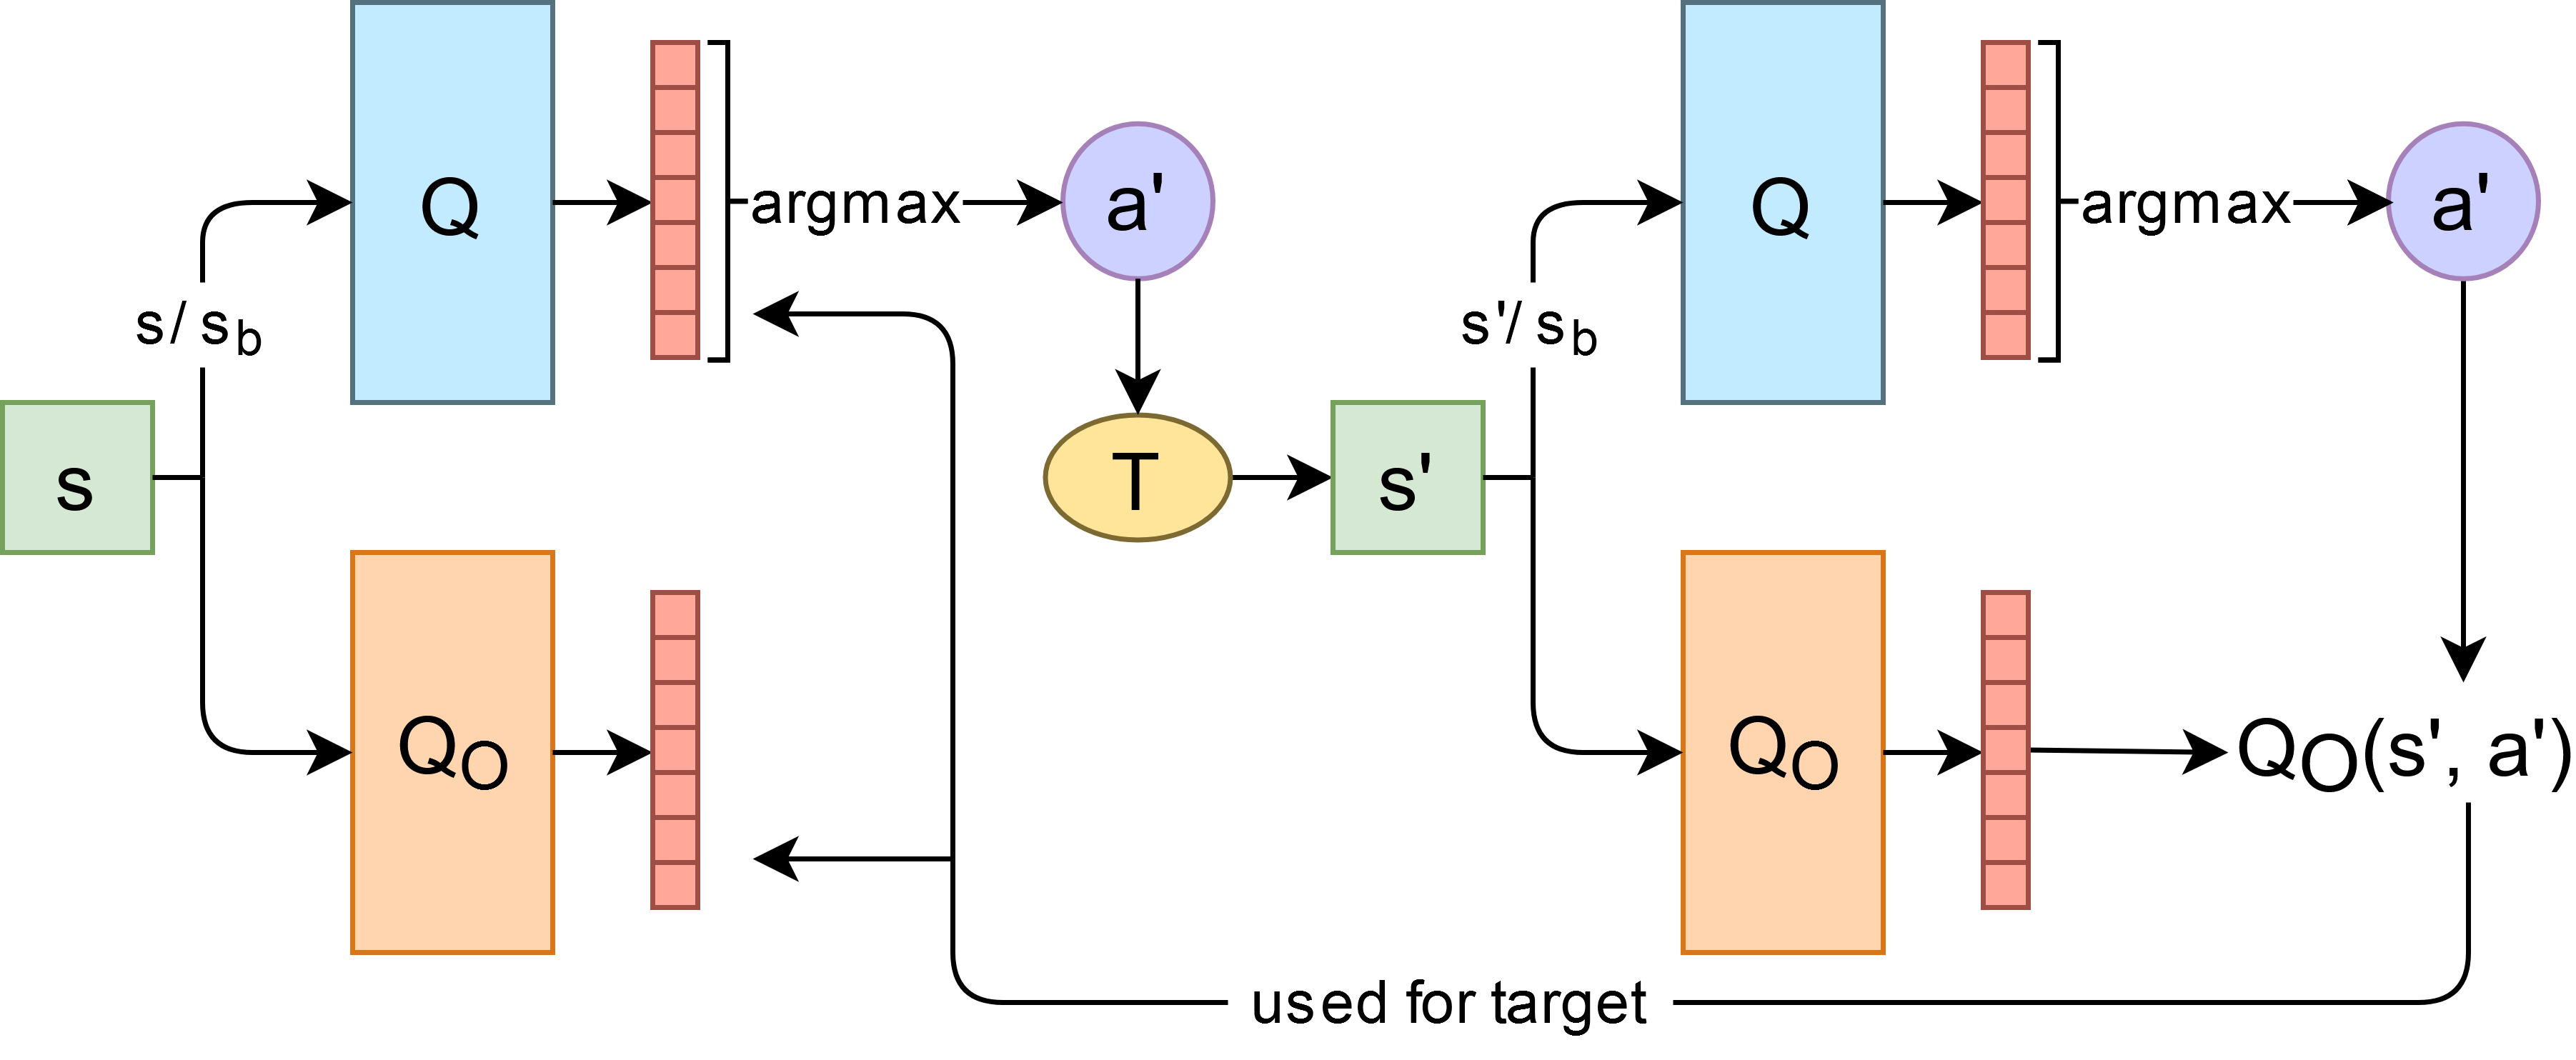
\includegraphics[width=1\textwidth]{images/images_part1/mnamenew.png}
\caption{One update of the modified DQN from (cite).}
\end{figure}

Those two variants of DQN and PPO have first been introduced in (PINTO) for robotics task and later studied theoretically to solve POMDPs (cite) in Baisero's work.
Baisero coined those approaches asymmetric reinforcement learning for POMDPs as an agent accesses full state information during the learning of a partially observable policy, hence using ``asymmetric'' information.
We study the connections between, learning decision tree policies for MDPs, and, POMDPs, extensively in the next chapter but for now we focus on reproducing the original results from (cite) in which POMDPs and asymmetric RL were not mentioned. 

Next, we present the precise experimental setup we use to reproduce the work of (cite) in order to study deep reinforcement learning of decision tree policies for the CartPole MDP.

\section{Experimental setup}
\subsection{(IB)MDP} 

We use the exact same MDP and associated IBMDP for our experiments as authors of (cite) except mentioned otherwise. Next, we describe in details the MDP and IBMDP used.

\paragraph{MDP} The problem at hand is the CartPole MDP. At each time step a learning agent observes the cart position velocity and the pole angle and angular velocity, and can take action to push the cart left or right. While the cart is roughly balanced, i.e., while the cart angle remains in some fixed range, the agent gets a positive reward.
If the cart is out of balance; the agent goes to an absorbing terminal state and gets 0 reward forever.
In practice, authors use the gymnasium \texttt{CartPole-v0} implementation (cite) of the CartPole MDP in which trajectories are truncated after 200 timesteps making the maximum cumulative reward over a trajectory to be 200.
Since the IBMDP definition requires the MDP state space to be a factor of bounded segments, authors bound the the state space of the CartPole MDP to be in $[-2.4, 2.4] \times [-2.4, 2.4] \times [-0.418, 0.418] \times [-0.418, 0.418]$.

\paragraph{IBMDP} Authors define the associated IBMDP with $\zeta=-0.01$ and parametric information gathering action space defined by $p=3$.
In addition we also try $\zeta=0.01$ and $p=2$.
The discount factor used by the authors is $\gamma=1$.

We potentially differ from the original paper setting in the way we handle maximum depth limiation. 
Indeed authors restrain the learning of policies to be equivalent to depth-2 trees but don't detail how they do so.
We hence try two different approaches as mentioned in the previous secion: terminating trajectories if the agent takes too much information gathering in a row or simply giving a reward of $-1$ to the agent everytime it takes an information gathering action past the depth limit.
This makes the transition or the reward function non markovian respectively as those operations are time dependent.

We will also try IBMDPs where we do not limit the maximum depth for completeness.

\subsection{Baselines}
\paragraph{Modified DQN} as mentioned above, authors use an asymmetric version (cite) of the DQN algorithm (cite).
We use the exact same hyperparameters for DQN as the authors when possible. 
We use the same layers width (128) and number of hidden layers (2), the same exploration strategy ($\epsilon$-greedy with linarly decreasing value $\epsilon$ between 0.5 and 0.05 during the first 10\% of the training),
the same replay buffer size ($10^6$) and the same number of transitions to be collected randomly before doing value updates ($10^5$).
We also try to use more exploartion during training (change the initial $\epsilon$ value to 0.9).
We use the same optimizer (RMSprop (cite) with hyperparmeter 0.95 and learning rate $2.5 \times 10^{-4}$) to update the $Q$-networks.

Authors did not share what DQN implementation they used so we used the stable-baselines3 one (cite).
Authors did not share what activations they used so we try both $\operatorname{tanh}()$ and $\operatorname{relu}()$. 

\paragraph{Modified PPO} for the modified PPO algorithm, we can exactly match the authors hyperparameters since they use the open source stable-baselines3 implementation of PPO.

Similarly to authors of (cite) we train DQN on 1 million timesteps and PPO on 4 million timesteps. For PPO, authors originally used 3.2 million timesteps but we rounded above: in practice this change should only be beneficial.

\paragraph{DQN and PPO} in addition to the above modified RL algorithms that learn a partially observable policy in an IBMDP equivalent to a decision tree policy for the CartPole MDP, we learn neural network policies $S\times O \rightarrow A\cup A_{info}$ and neural network $Q$-functions $S\times O \rightarrow \mathbb{R}^{|A\cup A_{info}|}$ using standard DQN and PPO on IBMDP.
We also apply those standard DQN and PPO to learn neural networks policies $S\times O \rightarrow A\cup A_{info}$ and neural network $Q$-functions $S\times O \rightarrow \mathbb{R}^{|A\cup A_{info}|}$ for the base CartPole MDP.
We can re-use the original paper (cite) hyperparameters to train the standard PPO and DQN. 

\paragraph{Indirect methods} we also learn decision tree policies by imitating the neural experts returned by standard PPO and DQN at different training stages.
In particular, when fitting decision trees to the greedy policy from $Q$-functions returned by DQN, we can use the VIPER variant of Alg (cite). This rescales each transition $(s, a)$ given by the expert by their importance in the future values $|\underset{\max}{a'}Q(s, a') - \underset{\max}{a''}Q(s, a'')|$ (see section of cite).
When fitting policies reuturned by PPO, unless we want to train an additional neural network to estimate $Q$-values, we are bound to use the Dagger (cite) algorithm (Alg (cite)) since PPO only returns a policy and a state-value function.

For each indirect method, we fit decision trees using the greedy tree classifier from scikit-learn with default hyperparameters and maximum depth of 2 to 10000 transitions collected by the neural experts.

We summarize hyperpameters for the IBMDP and for the learning algorithms in Tables (cite) and (cite).

\begin{table}[h]
    \centering
    \caption{IBMDP hyperparameters. We try 12 different IBMDPs. In \textcolor{green}{green} we highlight the hyperparameters from the original paper and in \textcolor{red}{red} we highlight the hyperparameter names for which author do not give information.}
    \begin{tabular}{ll}
    \toprule
    \textbf{Hyperparameter} & \textbf{Values}\\
    \midrule
    Discount factor $\gamma$ & \textcolor{green}{1} \\
    Information gathering actions parameter $p$ & 2, \textcolor{green}{3} \\
    Information gathering actions rewards $\zeta$ & \textcolor{green}{-0.01}, 0.01 \\
    \textcolor{red}{Depth control} & Done signal, negative reward, none \\ 
    \bottomrule
    \end{tabular}
    \end{table}

\begin{table}[h]
    \centering
    \caption{(Modified) DQN trained on $10^6$ timesteps. This gives four different instantiation of (modified) DQN. Hyperparameters not mentioned are stable-baselines3 default. In \textcolor{green}{green} we highlight the hyperparameters from the original paper and in \textcolor{red}{red} we highlight the hyperparameter names for which author do not give information.}
    \begin{tabular}{ll}
    \toprule
    \textbf{Hyperparameter} & \textbf{Values}\\
    \midrule
    Buffer size & \textcolor{green}{$10^6$} \\
    Random transitions before learning & \textcolor{green}{$10^5$} \\
    Epsilon stard & 0.9, \textcolor{green}{0.5} \\
    Epsilon end & \textcolor{green}{0.05} \\
    Exploration fraction & \textcolor{green}{0.1} \\
    Optimizer & \textcolor{green}{RMSprop ($\alpha = 0.95$)}\\
    Learning rate & \textcolor{green}{$2.5\times10^{-4}$}\\
    Networks architectures & \textcolor{green}{[128, 128]}\\
    \textcolor{red}{Networks activation} & $\operatorname{tanh()}$, $\operatorname{relu()}$\\
    \bottomrule
    \end{tabular}
    \end{table}

\begin{table}[h]
    \centering
    \caption{(Modified) PPO trained on $4\times10^6$ timesteps. This gives two different instantiation of (modified) PPO. Hyperparameters not mentioned are stable-baselines3 default. In \textcolor{green}{green} we highlight the hyperparameters from the original paper and in \textcolor{red}{red} we highlight the hyperparameter names for which author do not give information.}
    \begin{tabular}{ll}
    \toprule
    \textbf{Hyperparameter} & \textbf{Values}\\
    \midrule
    Steps between each policy gradient steps & \textcolor{green}{512} \\
    Number of minibatch for policy gradient updates & \textcolor{green}{4} \\
    Networks architectures & \textcolor{green}{[64, 64]}\\
    \textcolor{red}{Networks activations} & $\operatorname{tanh()}$, $\operatorname{relu()}$\\
    \bottomrule
    \end{tabular}
    \end{table}

\subsection{Metrics}

The key metric of this section is performance when controlling the CartPole after $t$ steps of learning.
Depending on what the underlying task is, we obtain this value during the training differently for each type of learning agent.
For modified RL algorithm that learn a partially observable policy or $Q$-function in an IBMPD, we periodically extract the policy or $Q$-function and use Alg 6 (cite) to extract a decision tree for the CartPole MDP. We then evaluate the tree on 10 independent trajectories in the MDP and report the mean cumulative reward.
For RL applied to IBMDPs, since we can't deploy learned policies directly to the base MDP as the state dimension mismatch, we evaluate those policy periodically to control an other IBMDP for the CartPole MDP where $\zeta=0$ ensuring that the cumulative IBMDP reward only corresponds to the reward for taking base actions.
Similarly we do 10 trajectories of the extracted policies in the evaluation IBMDP and report the average cumulative reward.

For RL applied directly to the base MDP we can just periodically extract the learned policies and evaluate them on ten trajectories of the base MDP.

Since imitation learning baselines do not train iteratively, we fit trees to neural experts trained for different duration on the base MDP. 
We then evaluate the imitated decision tree policy on ten trajectories on the CartPole base MDP.

Every single combination of IBMDP and modified RL instantiation is run 20 times.

For standard RL on IBMDP, we instantiate the IBMDP with original hyperparameters and depth control with negative rewards and we instantiate the RL algorithms with original hyperparameters and $\operatorname{tanh()}$ activations. Those two unique combinations are 20 times each.
For standard RL on the base MDP, we instantiate the standard RL with original hyperparameters and $\operatorname{tanh()}$ to.

Next, we present our results and discuss the reproducibility and limitations of the original approach presented in (cite).

\section{Results}
\begin{figure}
    \centering
    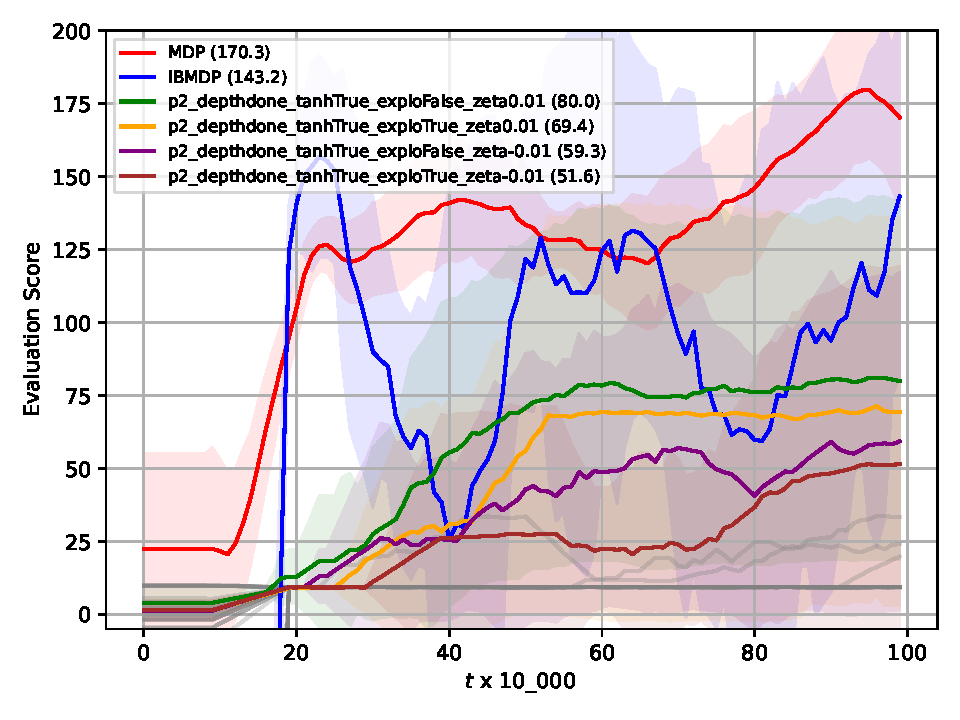
\includegraphics[width=0.8\textwidth]{images/images_part1/dqn.pdf}
    \caption{Variations of Modified DQN, DQN, VIPER and Dagger on CartPole IBMDP variations. We color the learning curves for DQN applied directly on CartPole and DQN applied on the IBMDP,
    We also color the Modified DQN variants that return the best decision tree policies for CartPole as well as in black the original paper Modified DQN (since there are multiple possible candidates for the original paper hyperparametrs, we choose to color the (Modified DQN variant, IBMDP variant) pair that resulted in the best decision tree policy on CartPole among the instances that could match the original paper).
    Dotted lines represent VIPER or Dagger trees performances on CartPole when fitted on neural expert returned by DQN on the base MDP at different learning states, i.e. each y-axis value of Dagger or Viper curves correspond to the performances of trees that were fitted on the greed policy from the $Q$-function which performance are the corresponding y-value on the red curve (DQN directly on CartPole).
    Shaded areas represent the standard deviation at each measure on the y-axis.}
\end{figure}

\begin{figure}
    \centering
    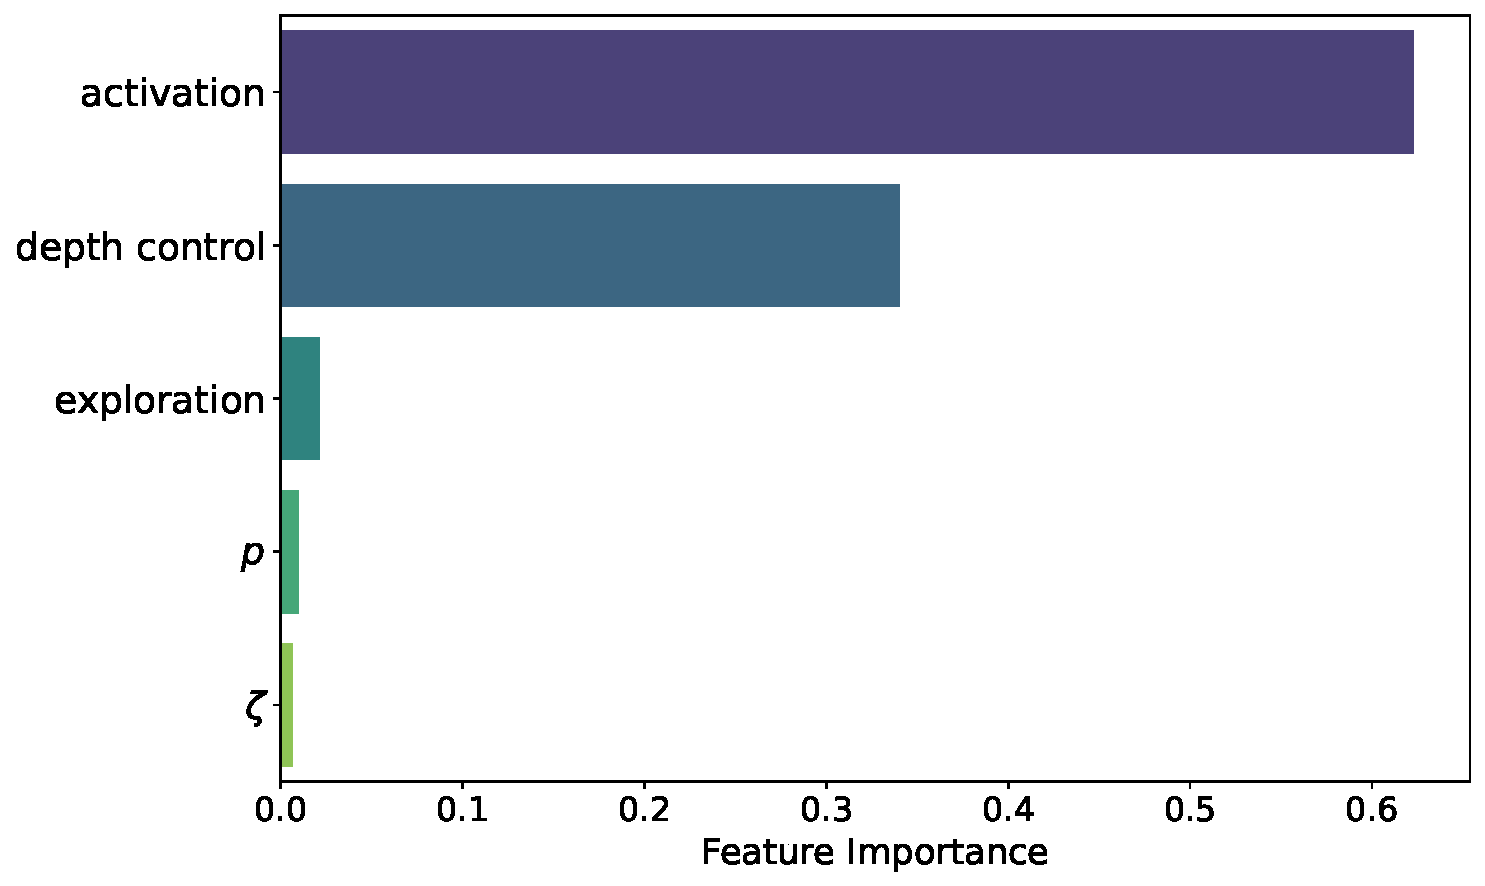
\includegraphics[width=0.8\textwidth]{images/images_part1/hyperparameter_importance_dqn.pdf}
    \caption{IBMDP and Modified DQN hyperparemters importance for predicting the learned decision tree policy perforance on CartPole using a RandomForest (cite).}
\end{figure}


\begin{figure}
    \centering
    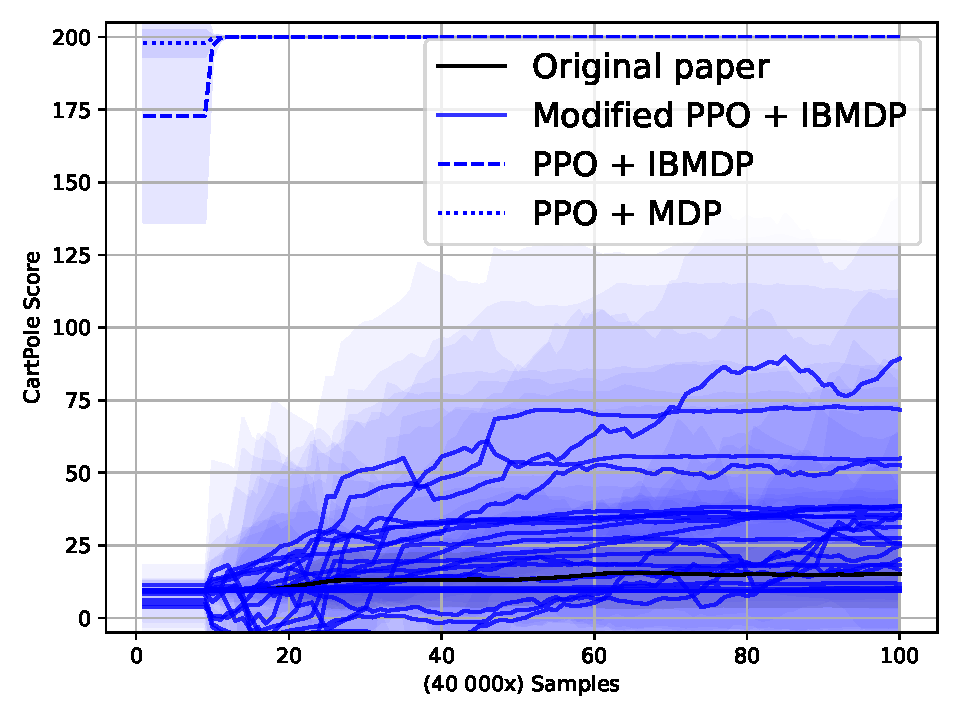
\includegraphics[width=0.8\textwidth]{images/images_part1/ppo.pdf}
    \caption{Variations of Modified PPO, PPO, VIPER and Dagger on CartPole IBMDP variations. We color the learning curves for PPO applied directly on CartPole and PPO applied on the IBMDP,
    We also color the Modified PPO variants that return the best decision tree policies for CartPole as well as in black the original paper Modified PPO (since there are multiple possible candidates for the original paper hyperparametrs, we choose to color the (Modified PPO variant, IBMDP variant) pair that resulted in the best decision tree policy on CartPole among the instances that could match the original paper).
    Dotted lines represent Dagger trees performances on CartPole when fitted on neural expert returned by PPO on the base MDP at different learning states, i.e. each y-axis value of the Dagger curve correspond to the performances of trees that were fitted on the greed policy from the $Q$-function which performance are the corresponding y-value on the red curve (DQN directly on CartPole).
    Shaded areas represent the standard deviation at each measure on the y-axis.}
\end{figure}

\begin{figure}
    \centering
    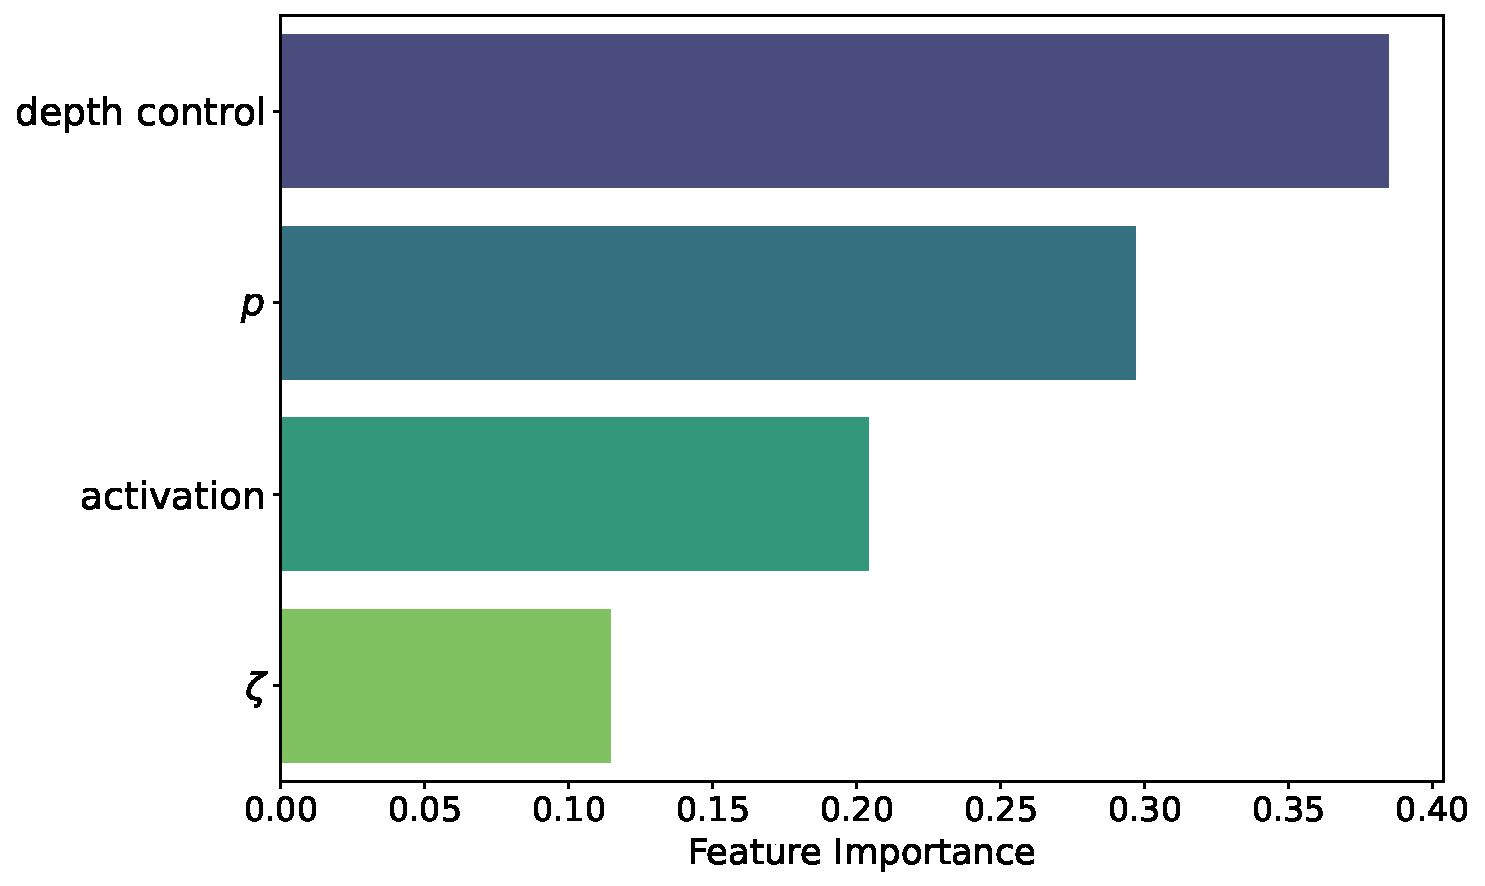
\includegraphics[width=0.8\textwidth]{images/images_part1/hyperparameter_importance_ppo.pdf}
    \caption{IBMDP and Modified PPO hyperparemters importance for predicting the learned decision tree policy perforance on CartPole using a RandomForest (cite).}
\end{figure}

\begin{figure}
    \centering
    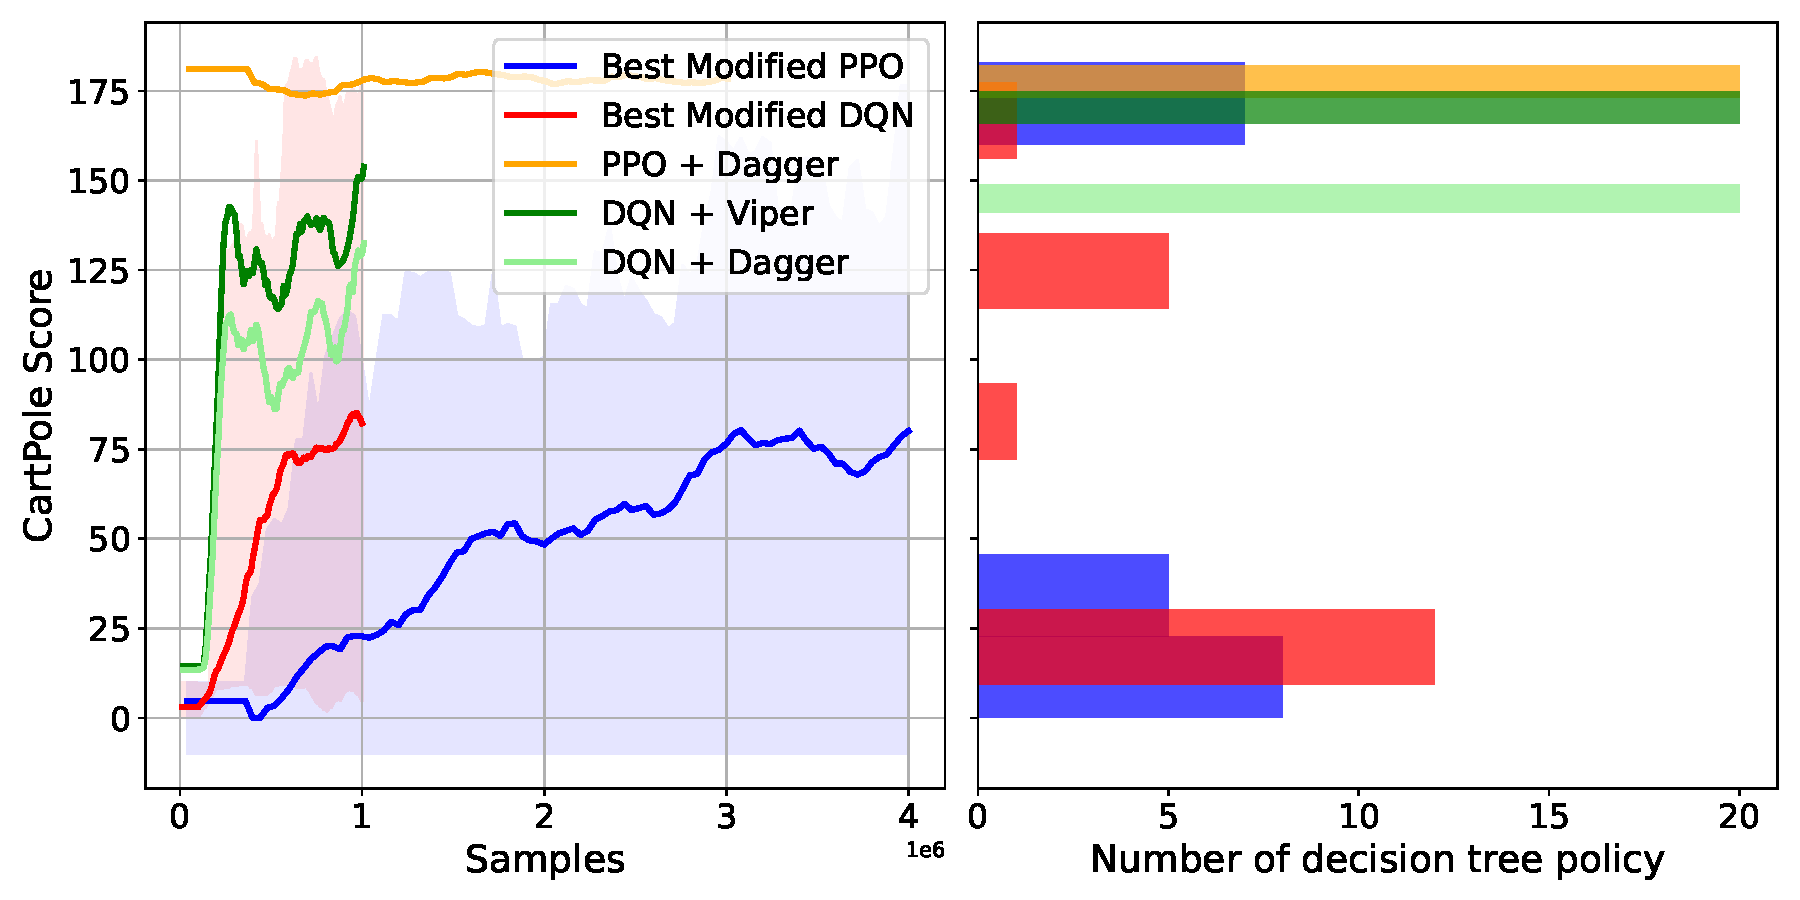
\includegraphics[width=0.8\textwidth]{images/images_part1/ppo_tree_study.pdf}
    \caption{(left) Mean performance of the best Modified PPO on the best IBMDP with shaded areas representing the min and max performance over the 20 seeds during training. (right) Histogram of the final decision tree policies performances.}
\end{figure}


\begin{figure}[htbp]
    \centering
    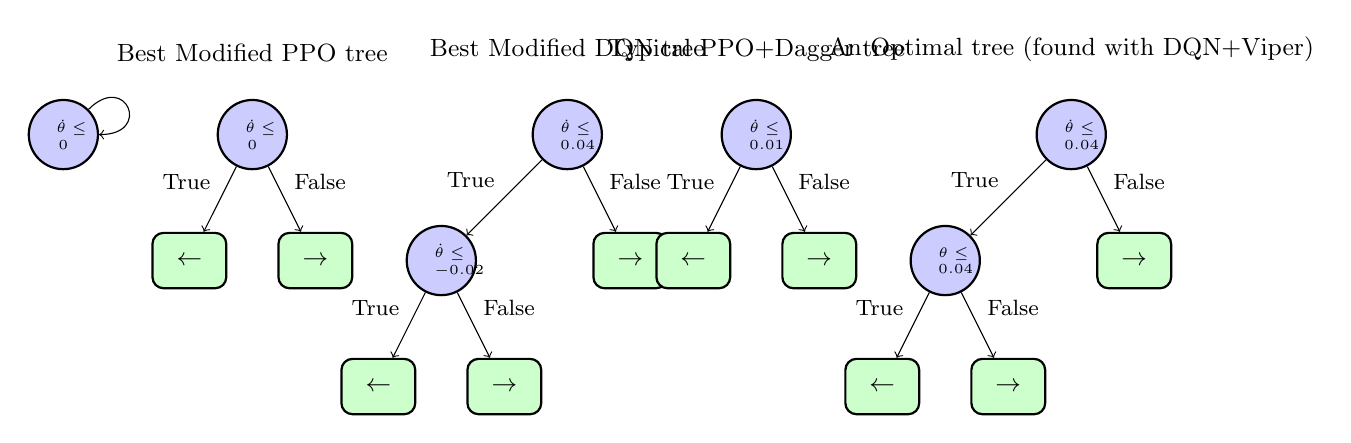
\begin{tikzpicture}[
        scale=0.8,
        decision/.style={circle, draw, thick, fill=blue!20, text width=0.5em, text centered, minimum height=2.5em, font=\tiny},
        leaf/.style={rectangle, draw, thick, fill=green!20, text width=2em, text centered, rounded corners, minimum height=2em, font=\small},
        edge_label/.style={font=\footnotesize, midway}
    ]

        \node[decision] (tree7_root) at (-3,0) {$\dot{\theta} \leq 0$};
        \draw[->] (tree7_root) to[out=45,in=0,looseness=5] (tree7_root);
        
        % Tree 4: if x <= 0.5 move right else move left
        \node[decision] (tree4_root) at (0,0) { $\dot{\theta}\leq 0$};
        \node[leaf] (tree4_right) at (-1,-2) {$\leftarrow$};
        \node[leaf] (tree4_left) at (1,-2) {$\rightarrow$};
        \draw[->] (tree4_root) -- (tree4_right) node[edge_label, above left] {True};
        \draw[->] (tree4_root) -- (tree4_left) node[edge_label, above right] {False};
        

        % Tree 7: if x <= 0.5 and y <= 0.5 move right else move down
        \node[decision] (tree7_root) at (5,0) {$\dot{\theta}\leq 0.04$};
        \node[decision] (tree7_y) at (3,-2) {$\dot{\theta}\leq -0.02$};
        \node[leaf] (tree7_right) at (2,-4) {$\leftarrow$};
        \node[leaf] (tree7_down) at (4,-4) {$\rightarrow$};
        \node[leaf] (tree7_down2) at (6,-2) {$\rightarrow$};
        \draw[->] (tree7_root) -- (tree7_y) node[edge_label, above left] {True};
        \draw[->] (tree7_root) -- (tree7_down2) node[edge_label, above right] {False};
        \draw[->] (tree7_y) -- (tree7_right) node[edge_label, above left] {True};
        \draw[->] (tree7_y) -- (tree7_down) node[edge_label, above right] {False};




        % Tree 4: if x <= 0.5 move right else move left
        \node[decision] (tree4_root) at (8,0) { $\dot{\theta}\leq 0.01$};
        \node[leaf] (tree4_right) at (7,-2) {$\leftarrow$};
        \node[leaf] (tree4_left) at (9,-2) {$\rightarrow$};
        \draw[->] (tree4_root) -- (tree4_right) node[edge_label, above left] {True};
        \draw[->] (tree4_root) -- (tree4_left) node[edge_label, above right] {False};
        

  
        % Tree 7: if x <= 0.5 and y <= 0.5 move right else move down
        \node[decision] (tree7_root) at (13,0) {$\dot{\theta}\leq 0.04$};
        \node[decision] (tree7_y) at (11,-2) {$\theta\leq 0.04$};
        \node[leaf] (tree7_right) at (10,-4) {$\leftarrow$};
        \node[leaf] (tree7_down) at (12,-4) {$\rightarrow$};
        \node[leaf] (tree7_down2) at (14,-2) {$\rightarrow$};
        \draw[->] (tree7_root) -- (tree7_y) node[edge_label, above left] {True};
        \draw[->] (tree7_root) -- (tree7_down2) node[edge_label, above right] {False};
        \draw[->] (tree7_y) -- (tree7_right) node[edge_label, above left] {True};
        \draw[->] (tree7_y) -- (tree7_down) node[edge_label, above right] {False};


        % Labels
        \node[above] at (0,1) {{\small Best Modified PPO tree}};
        \node[above] at (5,1) {{\small Best Modified DQN tree}};
        \node[above] at (8,1) {{\small Typical PPO+Dagger tree}};
        \node[above] at (13,1) {{\small An Optimal tree (found with DQN+Viper)}};

    \end{tikzpicture}
    \caption{Trees obtained by DRL against trees obtained with imitation.}
    \label{fig:trees-drl}
\end{figure}

Recall that implementing maximum tree depth control with a termination signal can break Markovianity of transitions while depth control with negative rewards can break Markovianity of the rewards, because in either case one has to keep track of the \textit{time} since the last base action.
We actually find that when $p+1$, the IBMDP information gathering space parameter, is a prime number, then as a direct consequence of the \textit{Chinese Reminder Theorem} (cite)(proof), the current tree is encoded in the current observation $o_t$. 
Hence, when $p+1$ is prime, we can control the depth throught trnasitions or rewards without tracking the time.
This could explain why on Figure (cite) the parameter $p$ is so important and why Modified DQN variants work better with $p=2$ than with the originally suggested $p=3$.


\section{Discussion}
We have shown that compared to learning non-interpretable policies for both the base MDP and the associated IBMDP, learning partially observable policies in IBMDP is very difficult even when learning policies corresponding to depth-2 decision trees for the simple CartPole task.
In the next chapter we down scale the learning algorithms to highlight the connexions between the above challenges and POMDP hardness results.